\section{Training data acquistion protocol}

The inclusion criteria for the subjects is that they must be healthy and able-bodied. The subjects will perform four different hand gestures: ulnar deviation, radial deviation, flexion and extension of the wrist, as shown in \figref{fig:handgest}. The order of the execution of the movements will be the same for each subject.

\begin{figure}[H]
	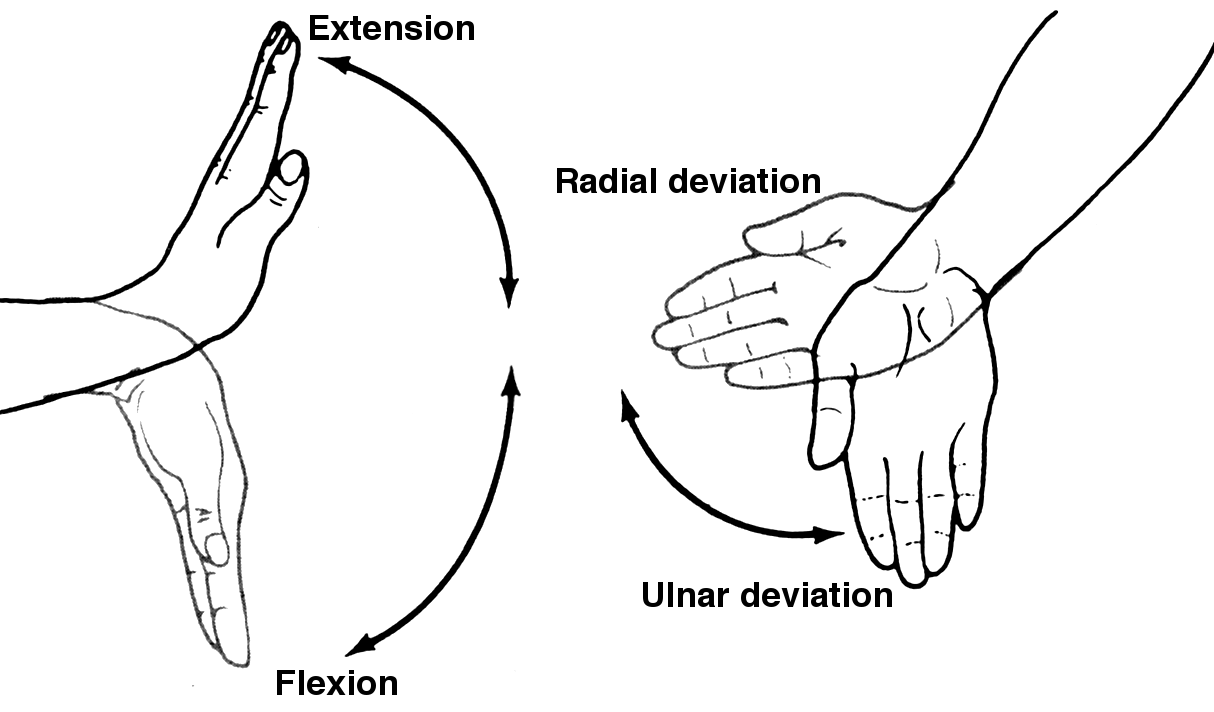
\includegraphics[width=.5\textwidth]{figures/Anatomy/wrist_move}  %<--but is not needed.
	\caption{Flexion, extension, radial and ulnar deviation of the hand. Modified from  \cite{hamilton2008}}
	\label{fig:handgest}  %<--give the figure a label, so you can reference!
\end{figure}

%In order to accomplish the study a Graphical User Interface $\left( GUI\right)$ had been created.The subjects of this study were familiar with the operation of the GUI.
At first the subject will have the baseline measured. The subject will have a relaxed forearm and hold the wrist in a neutral position. Afterwards each hand gesture will be performed as a fraction of the maximum voluntary contraction $\left( MVC\right)$ set as 30\% , 50\% and 80\%. The subjects will therefore initially be performing a MVC measure to be used as a reference measurement before the fraction of the MVC measures can be performed. The subjects will rest two minutes after the MVC measurement to avoid fatigue. This is done for each hand gesture. 

The acquisition of the fraction of the MVC of each hand gesture will consist of four chronological phases: a relaxed phase, a transition phase, a plateau phase and a relaxed phase, which will be depicted as a trapeze in a plot. The EMG of the subject will be depicted as a small circle in the plot, and the subject must follow the shape of the trapeze with the circle as best as possible. The recording of one fraction of MVC of one hand gesture will take ten seconds, where the phase with the highest contraction is four seconds. 
This procedure will be performed in three different limb positions, illustrated in the figure \figref{fig:limbpos}.

%maybe change the limb positions
\begin{figure}[H]                    
	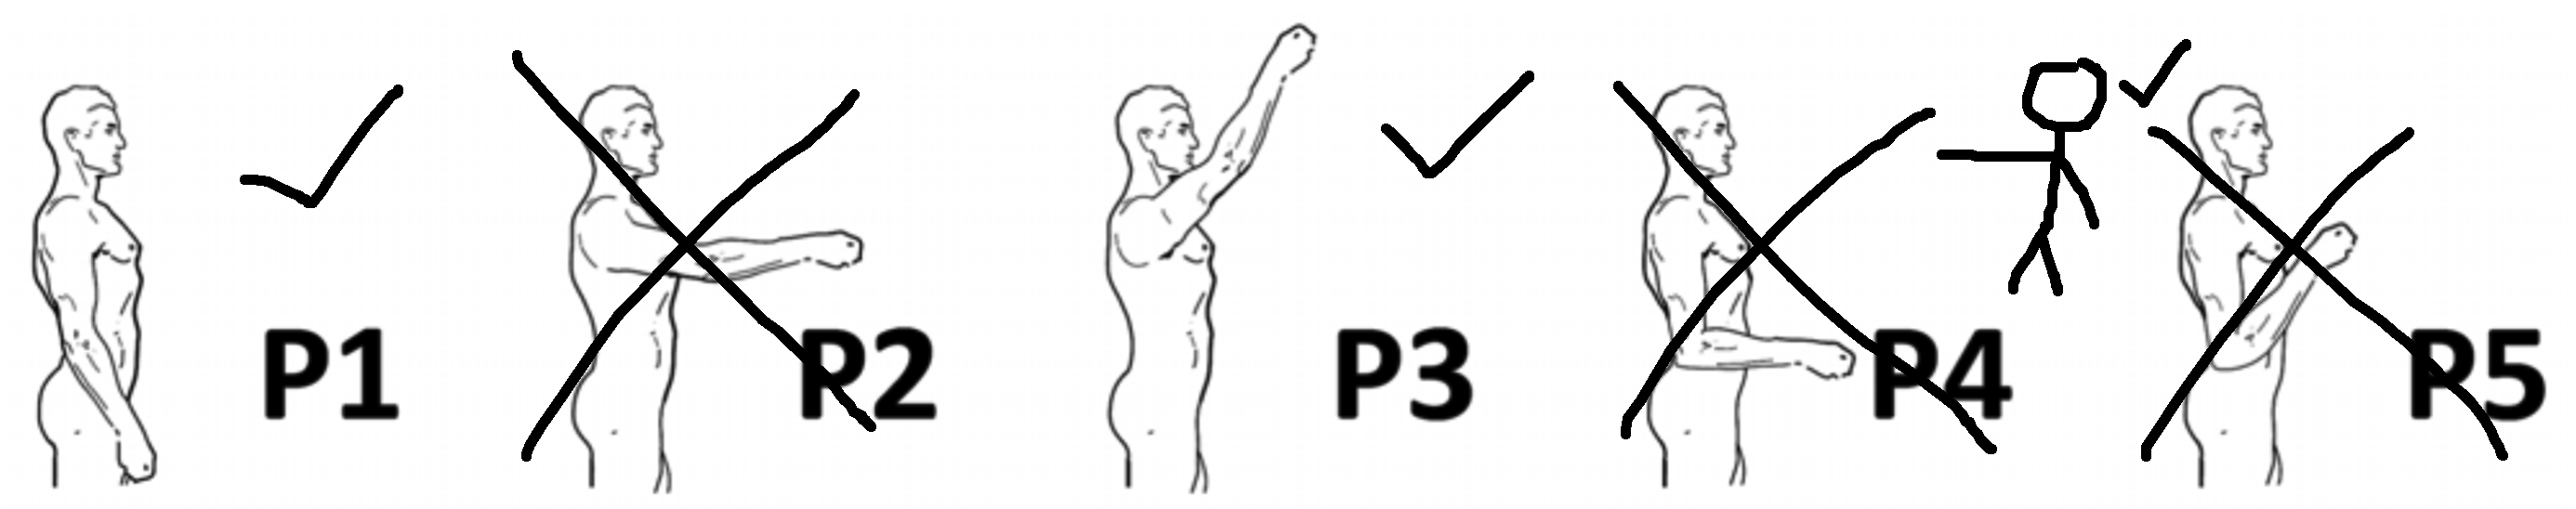
\includegraphics[width=1\textwidth]{figures/protocol/limb_position}  %<--but is not needed.
	\caption{The limb positions consist of: 1) Relaxed arm hanging at the side of the torso, 2) straight arm reaching horizontally away from the torso and 3) straight arm reaching up 45 degrees from vertical.}
	\label{fig:limbpos}  %<--give the figure a label, so you can reference!
\end{figure}

The subject will be given a relaxation period between trials in order to avoid shoulder fatigue.
Due to the fact that the hand gestures only consists of wrist movements, the subject must not move the fingers during the data acquisition.
The subjects will be in a standing position during the data acquisition procedure.
%time of rest?
Below is a table of the order at which each hand gesture will be performed, at which intensity and at which limb position. The table functions as a checklist for acquiring the training data.

%\begin{table}[h]
%	\centering
%\scalebox{.75}{
%		\begin{tabular}{|l|l|l|l|} 
%		\hline
%		& Limb 1 & Limb 2 & Limb 3  \\ \hline
%		\begin{tabular}[c]{@{}l@{}}Baseline\end{tabular} & & & & & \\ \hline
%		\begin{tabular}[c]{@{}l@{}}MVC\\ ulnar\end{tabular} & & & & & \\ \hline
%		\begin{tabular}[c]{@{}l@{}}25 \%\\ ulnar\end{tabular} & & & & & \\ \hline
%		\begin{tabular}[c]{@{}l@{}}50 \%\\ ulnar\end{tabular} & & & & & \\ \hline
%		\begin{tabular}[c]{@{}l@{}}75 \%\\ ulnar\end{tabular} & & & & & \\ \hline
%		\begin{tabular}[c]{@{}l@{}}MVC\\ radial\end{tabular} & & & & & \\ \hline
%		\begin{tabular}[c]{@{}l@{}}25 \%\\ radial\end{tabular} & & & & & \\ \hline
%		\begin{tabular}[c]{@{}l@{}}50 \%\\ radial\end{tabular} & & & & & \\ \hline
%		\begin{tabular}[c]{@{}l@{}}75 \%\\ radial\end{tabular} & & & & & \\ \hline
%		\begin{tabular}[c]{@{}l@{}}MVC\\ flex.\end{tabular} & & & & & \\ \hline
%		\begin{tabular}[c]{@{}l@{}}25 \%\\ flex.\end{tabular} & & & & & \\ \hline
%		\begin{tabular}[c]{@{}l@{}}50 \%\\ flex.\end{tabular} & & & & & \\ \hline
%		\begin{tabular}[c]{@{}l@{}}75 \%\\ flex.\end{tabular} & & & & & \\ \hline
%		\begin{tabular}[c]{@{}l@{}}MVC\\ ext.\end{tabular} & & & & & \\ \hline
%		\begin{tabular}[c]{@{}l@{}}25 \%\\ flex.\end{tabular} & & & & & \\ \hline
%		\begin{tabular}[c]{@{}l@{}}50 \%\\ flex.\end{tabular} & & & & & \\ \hline
%		\begin{tabular}[c]{@{}l@{}}75 \%\\ flex.\end{tabular} & & & & & \\ \hline
%		\begin{tabular}[c]{@{}l@{}}25 \%\\ ext.\end{tabular} & & & & & \\ \hline
%		\begin{tabular}[c]{@{}l@{}}50 \%\\ ext.\end{tabular} & & & & & \\ \hline
%		\begin{tabular}[c]{@{}l@{}}75 \%\\ ext.\end{tabular} & & & & & \\ \hline
%	\end{tabular}}
%
%	\caption{A checklist of the hand gestures each subject must perform and at which order.}
%	\label{tab:trainprotocol}
%\end{table}
\begin{table}[]
	\centering
	\caption{My caption}
	\label{my-label}
	\begin{tabular}{|l|l|l|l|}
		\hline
		& Limb 1 & Limb 2 & Limb 3 \\ \hline
		Baseline    &        &        &        \\ \hline
		MVC ulnar   &        &        &        \\ \hline
		25\% ulnar  &        &        &        \\ \hline
		50\% ulnar  &        &        &        \\ \hline
		75\% ulnar  &        &        &        \\ \hline
		MVC radial  &        &        &        \\ \hline
		25\% radial &        &        &        \\ \hline
		50\% radial &        &        &        \\ \hline
		75\% radial &        &        &        \\ \hline
		MVC flex.   &        &        &        \\ \hline
		25\% flex.  &        &        &        \\ \hline
		50\% flex.  &        &        &        \\ \hline
		75\% flex.  &        &        &        \\ \hline
		MVC ext.    &        &        &        \\ \hline
		25\% ext.   &        &        &        \\ \hline
		50\% ext.   &        &        &        \\ \hline
		75\% ext.   &        &        &        \\ \hline
	\end{tabular}
\end{table}